
\chapter{Introduction}
It is becoming increasingly important to educate the public about their energy usage.  With the current state of alternative energy research, it is impossible to support the entire world on renewable energy.  In order to ensure that current energy sources are still available for future generations, organizations from non-profits to utility providers have advocated energy conservation.  Some organizations specifically target younger students in order to instill energy conservation habits as they transition to the real world.

One approach to educating the younger generation is to hold college dormitory energy competitions.  The goal of these competitions is to have the residents of the dorm reduce their energy usage.  Typically, the dorm that reduces their energy use the most at the end of the competition is declared the winner.  Other smaller prizes can be awarded for accomplishing certain goals, like reducing energy usage by 10 percent in a week.  The overall energy reduction is determined either by having someone read the meters or using "smart meters" that are connected to the internet and can send out data.  Universities such as Duke (Eco-lympics) and the University of Wisconsin (Energy Apocalypse) have run competitions relating to energy conservation and awareness. 

These competitions usually involve more than just reducing energy usage.  The competition organizers also include activities that relate to energy conservation and are geared toward improving energy literacy and awareness.  Examples of activities range from viewing documentaries relating to conservation to attending recycling drives.  Participation in these activities and encouraging others to do the same can also be recognized and rewarded in the context of these dorm energy competitions.

\section{The Problem}

To aid in running the competition, many of these universities used web sites to display the resident's current usage.  While it is easy to create a content management system to display mostly static data (i.e. one that is only updated when someone reads the meter), dormitory residents are more motivated by real-time feedback\cite{oberlin-feedback}.  However, the development of such a system can be a complicated and/or expensive process.  Providing real-time feedback not only requires special meters that can communicate with other devices, but also requires software that can process the data and display the relevant information to the user.  Because of this, many organizations have turned to companies like Lucid Design Group that can provide this software and hardware at a cost.

However, Lucid Design Group's software only involves the visualization of energy data and does not involve energy awareness activities.  It is designed to be embedded within a website rather than a complete competition package.  Because of this, the software is unable to immediately provide user-related information.  For example, if a dorm resident wants to view their floor's energy usage, they must interact with the visualization to get the information that they need.  In the ideal case, the user would log in using their university credentials and then be able to immediately view their current standings.

As for energy activities, this type of information can be posted on a website.  However, organizers would also like to be able to track interest and participation in these activities so that users can be rewarded.  Users also could be more motivated to participate if they see others in their floor/dorm participating.  Adding in these functions go beyond what a standard content management system does.  Developing such a module for a competition would also take more time and/or resources.

\section{Makahiki}

The goal of Makahiki is to provide a complete software package for organizations that want to hold their own dorm energy competitions.  It will have the following features:

\begin{enumerate}
	\item Integration with WattDepot as a source of energy data.
	\item Produce visualizations of the energy data retrieved from WattDepot.
	\item Support for Central Authentication Service (CAS) for logging in and logging out of the system.
	\item The ability to create and track participation in activities, commitments, and goals.
	\item Integration with social networks such as Facebook and Twitter for displaying progress and standings.
\end{enumerate}

WattDepot\cite{wattdepot} is an open source web service in development here at the University of Hawaii at Manoa.  Its purpose is to collect electricity data from sources and to store it.  By combining Makahiki with WattDepot, competition organizers have an automated way of tracking the energy usage for buildings.  While compatible meters still need to be purchased, the software comes at no additional cost.  WattDepot also provides data at near-real time intervals, meaning that dorm residents can immediately see the results of their actions.

While WattDepot is able to collect all of the electricity data, the data still needs to be processed and presented to users in a visually appealing way.  Through the use Google Visualizations, electricity data can be presented in a way that is easy to understand and dynamic.  Users will be able to see their past and current electricity usage and be able to compare it to other floors.  Competition standings and goal status can also be displayed to users.

Students nowadays have university computer accounts that they use to access their email and other electronic resources.  Universities typically implement this using a CAS login, which requires the student to log in through a central university server before accessing protected resources.  By leveraging this student authentication, we are able to present energy data in the context of their dorm or floor.  We can also present an interface for students to create their own profile and participate in activities.

Because competitions involve more than just reducing energy usage, Makahiki will also have support for creating activities, commitments, and goals.  Activities can range from replacing light bulbs in a desk lamp to attending meetings by sustainability organizations.  Commitments are typically small "pledges" that dorm residents can accept, like committing to turning off the lights in the lounge.  Goals are actions that entire dorm floors participate in.  Goals can include reducing energy usage by ten percent or having all the members of a floor attend an event.  Dorm residents can participate in these items in order to gain points in the competition.

Furthermore, Makahiki will be configurable depending on the competition organizer's needs.  For instance, some organizations may wish to enter energy data manually since they cannot afford compatible smart meters.  Some organizations may wish to have a simple website for their competition without the added activities module.  These configurations are:

\begin{enumerate}
	\item Single page - A single page with news and charts.  The data for these charts can be either entered manually or retrieved from WattDepot.
	\item Tabbed interface - Includes sections for additional resources (i.e. links and videos) as well as energy data retrieved from WattDepot.
	\item Full Competition - Includes supplementary activities, commitments, and goals.  Also includes another tab for information about the competition.
\end{enumerate}

Finally, Makahiki will be open source.  This means that competition organizers can design the visual look of the application to fit their organization.  Also, advanced users can add or tweak modules in the application to fit their needs.

\section{Evaluating the Makahiki system}

The first step in evaluating the Makahiki system is to use it in our own dorm energy competition.  An initial version of Makahiki will be available for initial testing and review in the Summer of 2010.  Then, we will be holding a dorm energy competition here at the University of Hawaii at Manoa in October 2010 using both Makahiki and WattDepot.  Through the use of surveys, interviews, and/or log analysis, we hope to gain insight into how users will use the various features of Makahiki.

We also hope to provide an instance of Makahiki that looks similar to another dorm energy competition (for example, the Duke Eco-Olympics).  The purpose of this is to demonstrate the configuration options and how other universities can apply Makahiki to their own competition.

\section{Thesis Claims}

During the evaluation of Makahiki, we hope to answer the following questions:

\begin{enumerate}
	\item How effective is the site in influencing the energy usage habits of users?
	\item What components of Makahiki can we improve?
	\item How well does Makahiki support the potential needs of other energy competitions?
\end{enumerate}

\section{Proposal Structure}

Chapter 2 will discuss related works, which includes other dorm energy competitions.  Chapter 3 will describe the components of the Makahiki.  Chapter 4 describes our proposed evaluation procedure.  Finally, Chapter 5 includes the conclusion and provides a timeline for the work that is to be done to complete this project.

\chapter{Related Work}
\label{relatedwork}

The concept of holding dorm energy competitions is nothing new.  In fact, at least 25 institutions (including a private high school) have run dorm energy competitions.  This next section will discuss two of the more prominent dorm energy competitions; Duke and Oberlin.  We will then compare the features of the various universities.

\section{Other Dorm Energy Competitions}
\label{othercomps}

Duke held their first Eco-Olympics\cite{duke-eco-lympics} in 2002.  The Eco-Olympics not only involves energy conservation, but water conservation and waste reduction as well.  However, energy reduction plays a significant part in the competition as it is one of the largest components of the Eco-Olympics in terms of possible points.  Each week, the organizers get meter readings from the dorms and compare the readings with the dorm's respective baseline reading in order to calculate a per-capita reading.  This baseline reading is obtained in September, so it reflects usage when students are living in the dorm.   The key thing to note is that dorms are not directly competing against each other, as dorms vary in size and have differing energy requirements.  Also, the weekly readings are to provide feedback on how residents of each dorm are doing.  Points are only awarded at the end of the competition and the dorm with the lowest per-capita reading receives the full amount of points.

\begin{figure}[h]
	\includegraphics[scale=0.25]{images/duke-ecolympics.eps}
	\caption{Duke Eco-Olympics}
\end{figure}

The other major component of the Eco-Olympics is participation in events.  Dorms are awarded points based on the percent of residents who attend each event.  The amount of points for each event may vary, but the total points is comparable to the possible number of points for energy conservation.  These events can also involve conservation-related games.  The individuals participating in these games can also win prizes, providing additional incentive for dorm residents to participate.

Oberlin College in Ohio also runs dorm energy competitions.  Instead of going with manual meter readings, Oberlin has partnered with Lucid Design Group to create their Campus Resource Monitoring System\cite{oberlin-comp}.  The Campus Resource Monitoring System is active year-round and retrieves real time electricity and water usage from 26 buildings\cite{lucid-oberlin} on campus.  The system provides graphs and statistics and are presented to users in a clean and interactive way.

The first competition that used the Campus Resource Monitoring System proved to be a success.  A study conducted during the 2005 dorm energy competition found that dorms with real time feedback reduced their energy consumption by 55 percent while dorms with "medium resolution" feedback only reduced their energy usage by 32 percent\cite{oberlin-goals}.  In total, the competition saved 68,000 kW which translated to a savings of \textdollar5,100.

While Oberlin held yearly dorm energy competitions for some time, they had their first sustainability competition, called the Ecolympics, in March of 2008\cite{oberlin-history}.  The Ecolympics at Oberlin are run at about the same time as the dorm energy competition, but the two competitions are separate.  Dorms earn points for participation in events like attending environmentally themed lectures and film screenings\cite{oberlin-news}.  Depending on the event, participants can also win individual prizes.

\begin{figure}[h]
	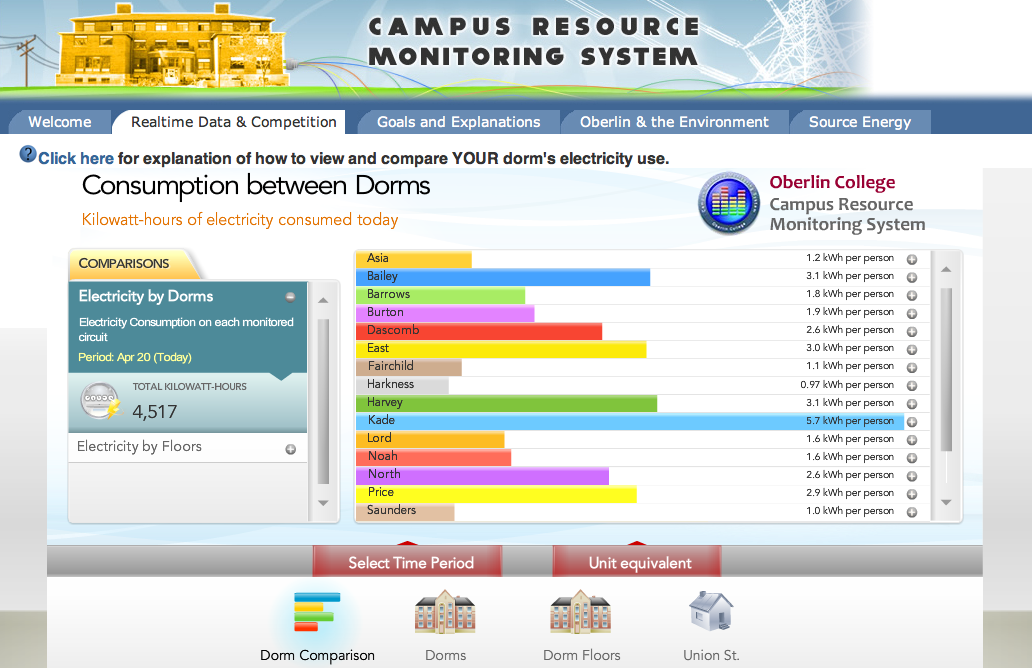
\includegraphics[scale=0.25]{images/oberlin-crms.eps}
	\caption{Oberlin College Campus Resource Management System}
\end{figure}

A few universities around the nation use Lucid Design Group's building dashboard for their dorm energy competition.  In addition to Oberlin College, Bowdoin College, St. John's University, Hamilton College, Boston College, and Elon University have all run dorm energy competitions through the use of Lucid Design Group's dashboard\cite{lucid-competitions} with great success.  Universities that do not use Lucid Design Group's dashboard typically go with a manual entry approach.

\begin{table}[h]
	\begin{tabular}{|l||l|l|l|l|}
		\hline
		Organization & Year Started & Competition Duration & Update Frequency & Activities \\
		\hline
		Duke University & 2002 & 1 month & Weekly & Yes \\
		Oberlin College & 2008 & 2 weeks & Real-Time & Yes \\
		Brandeis University & 2006 & 2 weeks & Weekly & No \\
		Bowdoin College & 2002 & 1 month & Real-Time & No \\
		Harvard & 1990\cite{harvard-greencup} & 7 months & Manual & Yes \\
		Indiana University & 2008\cite{indiana-first} & 1 month & Manual & No \\
		\hline
	\end{tabular}
	\caption{University dorm energy competition implementations}
	\label{feature-matrix}
\end{table}

\chapter{Makahiki}
\label{makahiki}

The proposed Kukui Cup System consists of two main components.  \autoref{webapp} describes the implementation of the web application.  \autoref{socialint} describes integration with popular social networks such as Facebook and Twitter.

\section{Web Application}
\label{webapp}

The current implementation of Makahiki is built using Django and Pinax.  Django\cite{django} is an open source web development framework implemented in Python.  Pinax\cite{pinax} is an open source platform built on Django that provides a set of reusable modules.  By using Pinax, we were able to start with a Django content management system and start building our unique modules right away.  Things like user accounts and profiles are created for us with little effort.

There are a few reasons why we chose Django and Pinax to implement Makahiki.  First, both are open source and thus other users who need to implement functionality can do so.  More importantly though, Django and Pinax provided us a lot of flexibility.  While we could have gone with a more popular content management system, these larger systems may not be flexible enough to support all of our needs.  Also, the process of extending such a large codebase would take additional time.  By going with Django, a general framework for creating web applications, we have the flexibility we desire.  And for the most part, we do not need to extend Django.  Instead, we just use the tools it provides to create the necessary modules for Makahiki.

\subsection{WattDepot Integration}

WattDepot is an open source web service that collects and stores energy usage data from meters.  The system is currently under development in the Collaborative Software Development Laboratory at the University of Hawaii at Manoa.  While instances of the service are hosted in the laboratory, organizations can choose to host their own instances.

There are several reasons why we want to support integration with WattDepot.  First, the data in WattDepot is accessible via a REST API\cite{wattdepot-rest}, meaning that external services can easily request and retrieve data from the system.  Also, WattDepot supports near-real time (sub-minute) update intervals, which is one of the reasons why competitions that use Lucid Design Group's Building Dashboard are so successful.  Other freely available solutions like Google PowerMeter\cite{google-powermeter} do not have this level of feedback.  

\subsection{Mobile Web Application}

Formatting the website for iPhone/Android users.

\section{Social Network Integration}
\label{socialint}

Integrating with Facebook and/or Twitter.

% \section{Other Notifications}
% \label{notifications}

\chapter{Evaluation}
\label{evaluation}

Focus groups, surveys, actual competition.

\chapter{Conclusion}
\label{conclusion}

It is our hope that this system will improve the participants energy literacy in a way that makes a lasting impact on their energy use outside of the competition.

\section{Anticipated Contributions}

We want to provide a system that integrates real-time energy data along with incentives for behavioral change.

\section{Thesis Timeline}

\begin{enumerate}
\item August 2010 - An early version of the Makahiki will be available for evaluation.
\item October 2010 - The competition will take place.
\end{enumerate}